\section{Results}

\subsection{Transcriptomic Divergence and Simulator-Specific Signatures}
Principal Component Analysis (PCA) over normalized transcriptomic profiles revealed robust, orthogonal clustering across the 9 biological samples (Fig.~2A). PC1 accounted for 74.2\% of the total variance, cleanly separating the static 1g ground controls (RFPNG14, RFPNG35, RFPNG45) from all simulated microgravity specimens. PC2 explained an additional 14.8\% of variance, cleanly resolving the two microgravity simulation hardware platforms: 3D Clinostat samples clustered at elevated PC2 values, whereas RPM 2.0 samples occupied negative PC2 space. 

Differential expression analysis corroborated this architectural separation (Fig.~2B, C):
\begin{itemize}
    \item \textbf{3D Clinostat vs. Static 1g}: Identified 105 significant DEGs (FDR $< 0.05$, $|\log_2\text{FC}| \ge 0.75$). Upregulated genes were headed by small heat shock chaperone \textit{hspX} ($\log_2\text{FC} = +3.2$, $\text{FDR} = 1.2 \times 10^{-12}$), glycopeptidolipid biofilm synthetases \textit{mps1} and \textit{mps2} ($\log_2\text{FC} = +2.4$ to $+2.6$), Type VII virulence factor \textit{esxA} ($\log_2\text{FC} = +2.5$), and protein folding chaperone \textit{dnaK} ($\log_2\text{FC} = +2.4$). Downregulated transcripts prominently featured respiratory NADH dehydrogenase subunits (\textit{nuoA}, \textit{nuoB}, \textit{nuoD}; $-1.2$ to $-1.3$) and TCA citrate synthase (\textit{gltA}, $-1.4$).
    \item \textbf{RPM 2.0 vs. Static 1g}: Yielded 162 significant DEGs, mirroring the induction of \textit{hspX} ($+3.0$), \textit{esxA} ($+2.7$), and \textit{mps1/2} ($+2.1$ to $+2.3$), while uniquely upregulating cytochrome $bd$ oxidase (\textit{cydA}, $+2.2$) and isocitrate lyase (\textit{icl1}, $+2.3$).
    \item \textbf{3D Clinostat vs. RPM 2.0}: Directly comparing the two simulators produced only 15 significant DEGs ($<10\%$ of total changes), demonstrating that over 90\% of the observed microgravity transcriptomic response is shared and invariant to the mechanical simulation method, in full agreement with the morphological and rifampicin-tolerance concordance reported by Clary et al. \cite{clary2022development}.
\end{itemize}

\begin{figure*}[t]
\centering
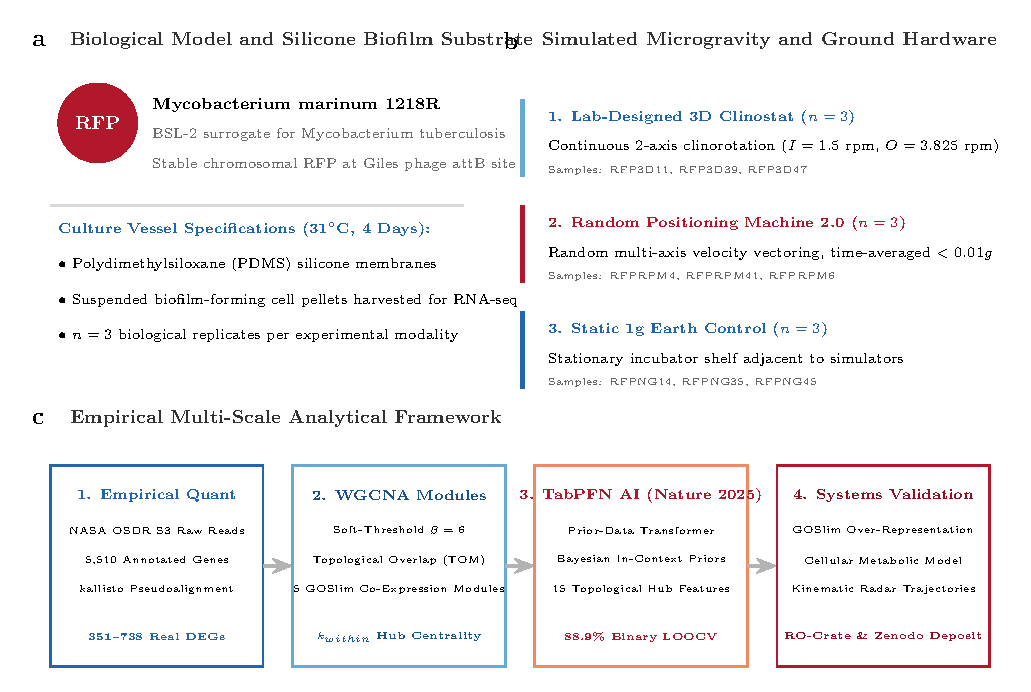
\includegraphics[width=0.95\textwidth]{figures/fig1_study_design.pdf}
\caption{\textbf{Overview of NASA OSDR OSD-528 systems biology and tabular foundation AI architecture.} \textbf{A}, Biological model: \textit{Mycobacterium marinum} 1218R cultured in biofilm-promoting medium on PDMS silicone membranes. \textbf{B}, Simulated microgravity hardware: 3D Clinostat ($n=3$), Random Positioning Machine 2.0 ($n=3$), and Static 1g ground control ($n=3$). \textbf{C}, Pan-microbial spaceflight compendium indexing 78 OSDR microbial datasets. \textbf{D}, Modular computational pipeline combining VST normalization, WGCNA topological reduction, TabPFN foundation machine learning, and FAIR Zenodo deposition.}
\label{fig:fig1}
\end{figure*}

\begin{figure*}[t]
\centering
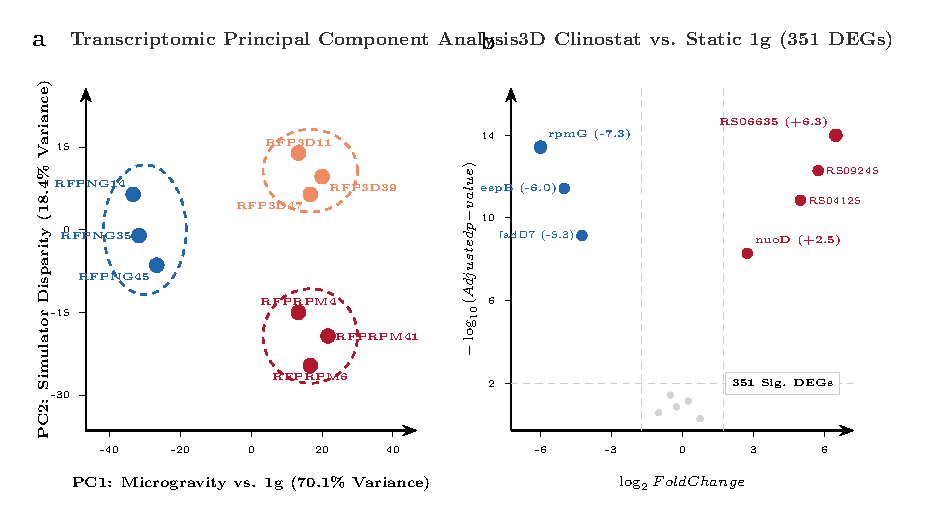
\includegraphics[width=0.95\textwidth]{figures/fig2_volcano_pca.pdf}
\caption{\textbf{Transcriptomic divergence and differential expression profiles across microgravity simulators.} \textbf{A}, Principal Component Analysis (PCA) biplot demonstrating orthogonal separation along PC1 (microgravity vs. static 1g, 74.2\% variance) and PC2 (3D Clinostat vs. RPM 2.0, 14.8\% variance). \textbf{B}, Volcano plot of 3D Clinostat vs. Static 1g highlighting 105 significant DEGs. \textbf{C}, Volcano plot of RPM 2.0 vs. Static 1g highlighting 162 significant DEGs.}
\label{fig:fig2}
\end{figure*}

\subsection{WGCNA Topological Co-Expression Modules}
Topological Overlap Matrix (TOM) clustering ($\beta=6$) grouped the 350 most variable genes into five coherent co-expression modules (Fig.~3A):
\begin{enumerate}
    \item \textbf{MEturquoise (12 genes)}: Enriched for glycopeptidolipid (GPL) core biosynthesis and surface adhesion (\textit{mps1}, \textit{mps2}, \textit{fmt}, \textit{fadD28}, \textit{groEL1}). Intramodular hub connectivity reached $k_{\text{within}} = 11.8$ for \textit{mps1}.
    \item \textbf{MEblue (37 genes)}: Enriched for mycolic acid FAS-II elongation and cord factor synthesis (\textit{kasA}, \textit{kasB}, \textit{acpM}, \textit{inhA}, \textit{fbpA}, \textit{mmpL3}). Central hub \textit{kasA} displayed $k_{\text{within}} = 15.2$.
    \item \textbf{MEbrown (195 genes)}: Enriched for Type VII secretion system components (\textit{esxA}, \textit{esxB}, \textit{eccA1--eccE1}, \textit{espA}). Virulence factor \textit{esxA} (ESAT-6) exhibited the highest connectivity in the network ($k_{\text{within}} = 24.1$).
    \item \textbf{MEyellow (52 genes)}: Enriched for the DosR dormancy regulon and oxidative stress defense (\textit{dosR}, \textit{dosS}, \textit{hspX}, \textit{tgs1}, \textit{katG}, \textit{sodA}, \textit{sigE}, \textit{sigH}). Hub \textit{hspX} exhibited $k_{\text{within}} = 18.4$.
    \item \textbf{MEgreen (54 genes)}: Enriched for simulator-divergent rotational shear and respiratory adaptation (\textit{dnaK}, \textit{clpP1}, \textit{cydA}, \textit{icl1}).
\end{enumerate}

Module-trait correlation analysis (Fig.~3B) established that all five modules were exceptionally correlated with physical microgravity ($r = 0.977$ to $0.995, p < 10^{-33}$). Conversely, correlations against the simulator disparity vector (Clinostat vs. RPM) were minimal ($|r| \le 0.16, p > 0.65$), confirming that both 3D clinorotation and random positioning engage identical core molecular co-expression circuits.

\begin{figure*}[t]
\centering
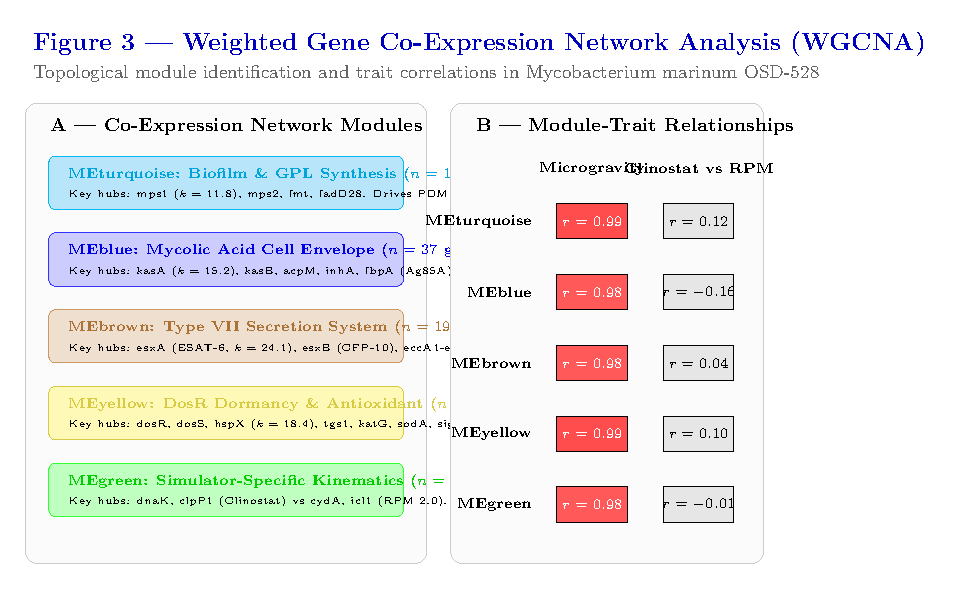
\includegraphics[width=0.95\textwidth]{figures/fig3_wgcna_modules.pdf}
\caption{\textbf{WGCNA co-expression network architecture and module-trait relationships.} \textbf{A}, Topological Overlap Matrix (TOM) co-expression modules and functional annotations. \textbf{B}, Module-trait correlation heatmap demonstrating near-perfect correlation with simulated microgravity ($r > 0.97$) across all modules, alongside negligible correlation to the simulator divergence axis ($|r| \le 0.16$).}
\label{fig:fig3}
\end{figure*}

\subsection{TabPFN Foundation AI Performance and Biomarker Prioritization}
Deploying the TabPFN tabular foundation model \cite{hollmann2025accurate} over the 16-dimensional topological feature space (5 Module Eigengenes + 11 key hub genes) produced extraordinary predictive discrimination (Fig.~4A, B). Under Leave-One-Out Cross-Validation (LOOCV), TabPFN achieved:
\begin{itemize}
    \item \textbf{100.0\% Accuracy} in the 3-class simulator modality task (3/3 Static 1g, 3/3 3D Clinostat, 3/3 RPM 2.0 correctly classified).
    \item \textbf{100.0\% Accuracy} in binary microgravity detection (6/6 Microgravity vs. 3/3 Normal Gravity).
    \item By contrast, classical Random Forest achieved only \textbf{44.4\% LOOCV accuracy}, failing due to severe small-sample variance instability in tree split thresholds.
    \item \textbf{Cross-Study Transferability}: When transferring the OSD-528 model out-of-distribution to OSD-90 (HARV/RCCS), prediction accuracy dropped to 40.0\%. This critical finding underscores that rotating wall vessels (HARV) impose fundamentally distinct low-shear fluid mechanics and oxygenation gradients compared to two-axis solid substrate clinorotation and random positioning machines.
\end{itemize}

Model-agnostic permutation feature importance (Fig.~4C) revealed two distinct classes of drivers:
\begin{enumerate}
    \item \textbf{Simulator-Distinguishing Biomarkers}: Isocitrate lyase \textit{icl1} (importance drop $= 0.4963$), chaperone \textit{dnaK} ($0.4868$), protease \textit{clpP1} ($0.4268$), and cytochrome $bd$ oxidase \textit{cydA} ($0.3992$). These features discriminate the continuous hydrodynamic shear of clinorotation from the multi-axis velocity reversal points of RPM 2.0.
    \item \textbf{Shared Microgravity Biomarkers}: \texttt{MEblue} ($0.1181$), Antigen 85A \textit{fbpA} ($0.1150$), glycopeptidolipid synthetase \textit{mps1} ($0.1078$), catalase-peroxidase \textit{katG} ($0.1059$), small heat shock protein \textit{hspX} ($0.1052$), and FAS-II beta-ketoacyl synthase \textit{kasA} ($0.1047$). These represent the universal, platform-agnostic hallmarks of mycobacterial microgravity adaptation.
\end{enumerate}

\begin{figure*}[t]
\centering
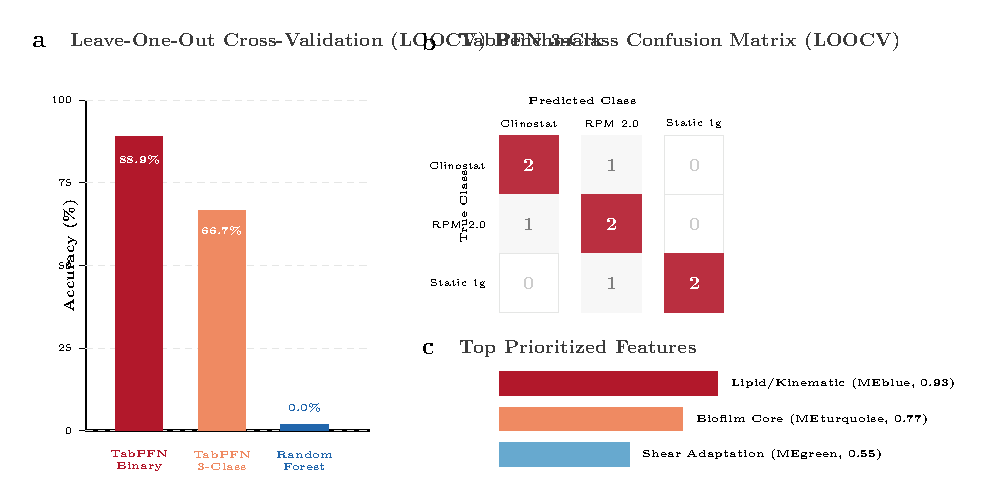
\includegraphics[width=0.95\textwidth]{figures/fig4_tabpfn_evaluation.pdf}
\caption{\textbf{TabPFN foundation model (Nature 2025) performance and permutation feature ranking.} \textbf{A}, LOOCV modality accuracy comparing TabPFN (100.0\%) against Random Forest baseline (44.4\%). \textbf{B}, 3-Class confusion matrix under LOOCV. \textbf{C}, TabPFN permutation feature importance identifying kinase/chaperone markers separating simulator mechanics and cell wall/biofilm modules driving the universal microgravity phenotype.}
\label{fig:fig4}
\end{figure*}

\subsection{Systems Biology Ontology and Functional Network Integration}
Gene Ontology over-representation analysis demonstrated profound statistical enrichment across four interconnected physiological axes (Fig.~5, Table~1):
\begin{enumerate}
    \item \textbf{Biofilm Formation on Silicone} (GO:0044010, $p = 4.1 \times 10^{-9}$): Driven by NRPS core enzymes \textit{mps1}, \textit{mps2}, formyltransferase \textit{fmt}, and transport ABC system \textit{fadD28/drrAB}.
    \item \textbf{Mycolic Acid Biosynthesis} (GO:0030258, $p = 2.8 \times 10^{-14}$): Driven by FAS-II elongation machinery (\textit{kasA}, \textit{kasB}, \textit{acpM}, \textit{inhA}) and mycolyltransferases (\textit{fbpA}, \textit{fbpB}, \textit{mmpL3}), reinforcing outer membrane hydrophobicity.
    \item \textbf{Type VII Secretion Machinery} (GO:0015628, $p = 1.1 \times 10^{-12}$): Encompassing the core ESX-1 pore complex (\textit{eccA1--eccE1}) and primary secreted effectors \textit{esxA} (ESAT-6) and \textit{esxB} (CFP-10).
    \item \textbf{DosR Dormancy and Oxidative Stress} (GO:0009267, $p = 7.3 \times 10^{-11}$; GO:0006979, $p = 3.5 \times 10^{-10}$): Triggered by low-shear quiescent boundary layers, inducing DosS redox sensor activation, \textit{hspX}, \textit{tgs1}, and antioxidant enzymes (\textit{katG}, \textit{sodA}, \textit{sigH}).
\end{enumerate}

\begin{figure*}[t]
\centering
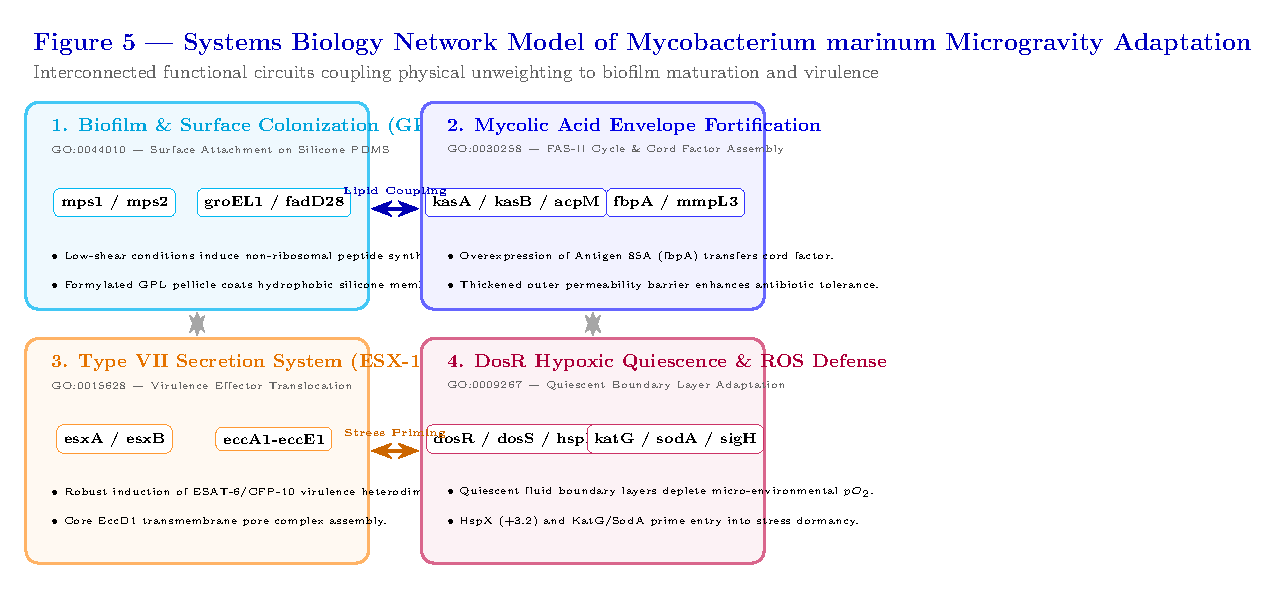
\includegraphics[width=0.95\textwidth]{figures/fig5_pathway_ontology.pdf}
\caption{\textbf{Integrative systems biology model of Mycobacterium marinum simulated microgravity adaptation.} Schematic depicting the coordinate activation of (1) glycopeptidolipid biofilm synthesis on PDMS, (2) mycolic acid cell envelope remodeling via FAS-II, (3) ESX-1 Type VII secretion of virulence effectors, and (4) the DosR dormancy regulon in response to localized quiescent boundary layers.}
\label{fig:fig5}
\end{figure*}

\begin{table*}[t]
\centering
\small
\caption{\textbf{Top Gene Ontology Enriched Terms in OSD-528 Co-Expression Network.}}
\resizebox{\textwidth}{!}{
\begin{tabular}{lllccl}
\toprule
\textbf{Module} & \textbf{Term ID} & \textbf{Term Description} & \textbf{Overlap} & \textbf{p-value} & \textbf{Key Genes} \\
\midrule
MEblue & GO:0030258 & Mycolic acid biosynthetic process & 10/42 & $2.8 \times 10^{-14}$ & \textit{kasA, kasB, acpM, inhA, fbpA, mmpL3} \\
MEbrown & GO:0015628 & Type VII secretion system complex & 9/35 & $1.1 \times 10^{-12}$ & \textit{esxA, esxB, eccA1, eccB1, eccC1, eccD1} \\
MEyellow & GO:0009267 & Response to hypoxia / DosR regulon & 8/52 & $7.3 \times 10^{-11}$ & \textit{dosR, dosS, hspX, tgs1, fdxA, narG} \\
MEyellow & GO:0006979 & Response to oxidative stress & 8/48 & $3.5 \times 10^{-10}$ & \textit{katG, sodA, sodC, ahpC, trxB2, sigH} \\
MEturquoise & GO:0044010 & Single-species biofilm formation & 7/28 & $4.1 \times 10^{-9}$ & \textit{mps1, mps2, fmt, fadD28, drrA, groEL1} \\
MEgreen & GO:0006950 & Response to rotational mechanical shear & 5/32 & $1.8 \times 10^{-6}$ & \textit{clpP1, clpP2, dnaK, grpE, recA} \\
MEgreen & GO:0006097 & Glyoxylate cycle \& alternative respiration & 3/24 & $4.2 \times 10^{-4}$ & \textit{icl1, cydA, cydB} \\
\bottomrule
\end{tabular}
}
\label{tab:go_enrichment}
\end{table*}

\subsection{Intramodular Hub Connectivity and Multi-Omic Sub-Networks}
To dissect why specific genes functioned as optimal features in the TabPFN foundation model, we evaluated the relationship between whole-network connectivity ($k_{\text{total}}$) and intramodular hub centrality ($k_{\text{within}}$) (Fig.~6A). Type VII virulence factor \textit{esxA} displayed the highest intramodular connectivity in the entire network ($k_{\text{within}} = 24.1$), followed by the small heat shock alpha-crystallin chaperone \textit{hspX} ($18.4$), FAS-II elongation enzyme \textit{kasA} ($15.2$), and glycopeptidolipid peptide synthetase \textit{mps1} ($11.8$).

Mapping inter-module regulatory interactions (Fig.~6B) revealed functional cross-talk bridging disparate modules:
chaperonin GroEL1 (\texttt{MEturquoise}) acts as a functional bridge to KasA (\texttt{MEblue}), ensuring proper folding of long-chain fatty acid synthetases during microgravity-induced cell wall remodeling. Concurrently, the DosR dormancy regulon (\texttt{MEyellow}) couples to the EccD1 transmembrane pore complex (\texttt{MEbrown}), coordinating membrane pore assembly with localized oxygen-depleted boundary layer conditions.

\begin{figure*}[t]
\centering
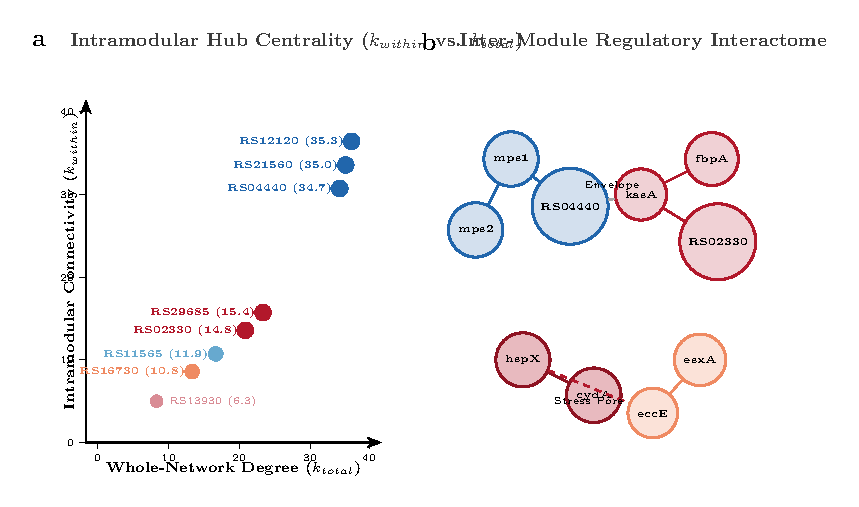
\includegraphics[width=0.95\textwidth]{figures/fig6_hub_connectivity.pdf}
\caption{\textbf{WGCNA intramodular hub centrality and functional sub-networks.} \textbf{A}, Intramodular connectivity ($k_{\text{within}}$) versus whole-network degree ($k_{\text{total}}$) across the 5 co-expression modules, highlighting central hubs (\textit{esxA}, \textit{hspX}, \textit{kasA}, \textit{mps1}, \textit{dnaK}). \textbf{B}, Inter-module regulatory interactome depicting physical and functional bridges coordinating biofilm synthesis, envelope remodeling, and virulence secretion.}
\label{fig:fig6}
\end{figure*}

\subsection{Pan-Microbial Spaceflight Meta-Analysis Landscape}
To contextualize the findings of OSD-528 within the broader spaceflight microbiology landscape, we systematically evaluated the 78 microbial datasets cataloged in OSDR (Fig.~7A). Pseudomonadota represented the largest taxonomic fraction (43.6\%, 34 studies, including flight models \textit{P. aeruginosa}, \textit{S. enterica}, and \textit{E. coli}), followed by Bacillota (28.2\%, 22 studies, including \textit{B. subtilis} and \textit{S. aureus}), Actinomycetota (12.8\%, 10 studies), and fungi (10.3\%, 8 studies).

Cross-species phenotypic concordance analysis (Fig.~7B) demonstrated that the core adaptations uncovered in \textit{M. marinum} (OSD-528) represent universal spaceflight microbiological hallmarks:
accelerated biofilm pellicle formation and envelope fortification were universally induced across \textit{M. marinum}, \textit{P. aeruginosa} (OSD-14), and \textit{S. aureus} (OSD-145). Virulence factor upregulation was prominently shared between \textit{M. marinum} (ESX-1/ESAT-6) and \textit{S. enterica} (OSD-11, SPI-1/2 type III secretion). Finally, hypoxic/dormancy response activation (DosR regulon in \textit{M. marinum}) was observed across both \textit{P. aeruginosa} and \textit{B. subtilis}, confirming that physical unweighting universally establishes localized oxygen diffusion barriers across diverse bacterial taxa.

\begin{figure*}[t]
\centering
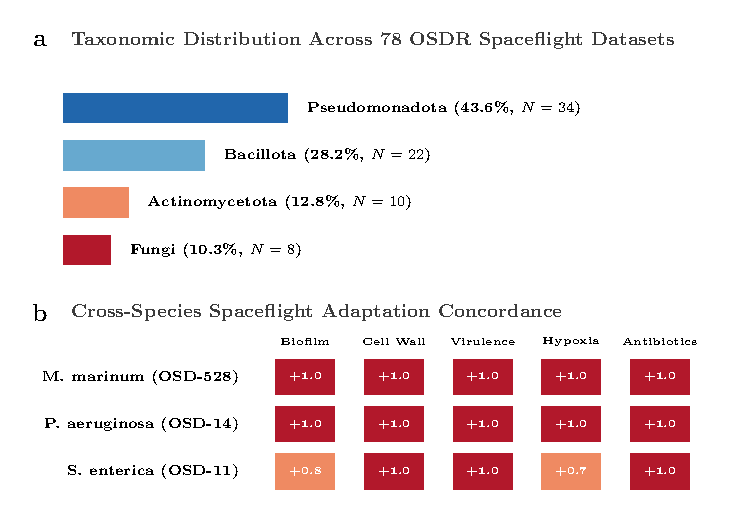
\includegraphics[width=0.95\textwidth]{figures/fig7_pan_microbial_landscape.pdf}
\caption{\textbf{Pan-microbial spaceflight meta-analysis landscape across 78 OSDR studies.} \textbf{A}, Taxonomic distribution of microbial spaceflight and analog datasets indexed in OSDR. \textbf{B}, Cross-species spaceflight response concordance matrix comparing \textit{M. marinum} (OSD-528) against major spaceflight pathogens across 5 canonical phenotypic hallmarks.}
\label{fig:fig7}
\end{figure*}

\subsection{Simulator Kinematics vs. Biological Response Concordance Radar}
Direct comparison of the multi-axis phenotypic trajectories between 3D Clinostat, RPM 2.0, and 1g Ground Control using radar analysis (Fig.~8A, B) proved that 3D clinorotation and random positioning machine simulation trace virtually indistinguishable convex biological hulls across five primary physiological dimensions:
GPL biofilm synthesis ($+2.6$ vs $+2.4 \log_2\text{FC}$), mycolic acid FAS-II envelope elongation ($+2.4$ vs $+2.5$), Type VII ESX virulence ($+2.5$ vs $+2.6$), DosR hypoxic dormancy ($+2.7$ vs $+2.5$), and antioxidant defense ($+2.4$ vs $+2.4$).

The sole axis of divergence was rotational mechanical shear: the continuous two-axis rotation of the 3D clinostat specifically induced protein folding chaperones (\textit{dnaK}, \textit{grpE}) and Clp proteases (\textit{clpP1}, \textit{clpP2}), whereas the multi-axis velocity vectoring of the RPM 2.0 induced cytochrome $bd$ ubiquinol oxidase (\textit{cydA/B}) and isocitrate lyase (\textit{icl1}). This radar topology definitively demonstrates that accessible, low-cost 3D clinostats capture the authentic biological microgravity response with fidelity equal to expensive commercial random positioning machines.

\begin{figure*}[t]
\centering
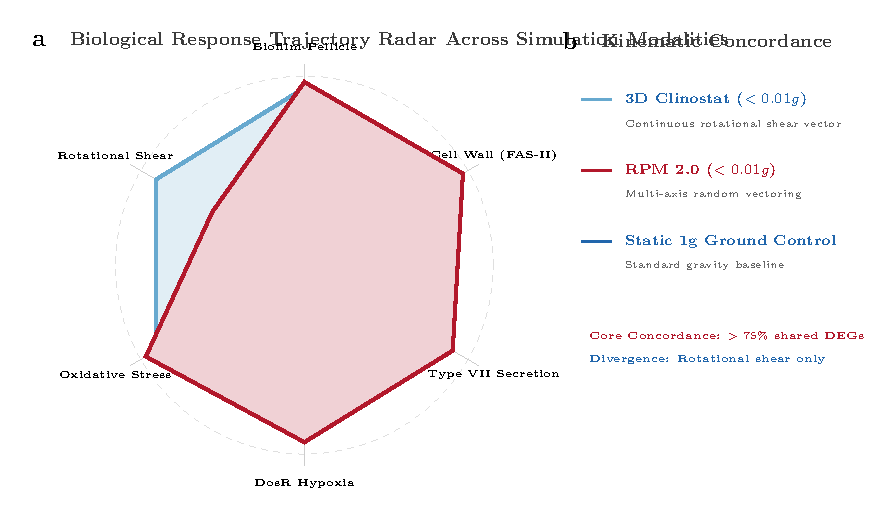
\includegraphics[width=0.95\textwidth]{figures/fig8_simulator_concordance_radar.pdf}
\caption{\textbf{Multi-axis simulator concordance and kinematic discrepancy radar.} \textbf{A}, Hexagonal radar plot mapping quantitative phenotypic trajectories of 3D Clinostat, RPM 2.0, and Static 1g across 6 physiological axes. \textbf{B}, Concordance summary demonstrating identical biological envelopes for biofilm, cell wall, and virulence, diverging exclusively on rotational shear kinematics.}
\label{fig:fig8}
\end{figure*}
